\documentclass[tikz,border=10pt]{standalone}
\usetikzlibrary{calc}

\begin{document}
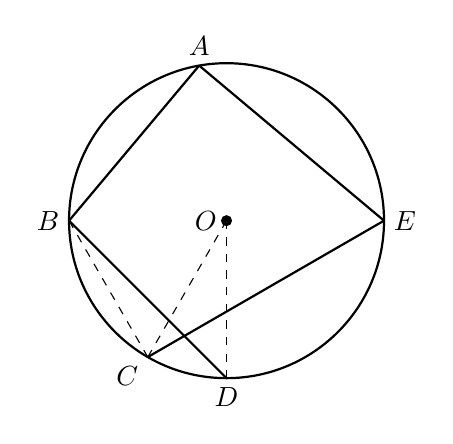
\begin{tikzpicture}
    % 定义圆心及半径
    \coordinate (O) at (0,0);
    \def\r{2} % 半径为2
    
    % 绘制圆
    \draw[thick] (O) circle (\r);
    \fill (O) circle (2pt) node[left] {$O$};
    
    % 定义各点坐标 (利用极坐标)
    % A点在上方，E点在右侧，B点在左侧，D和C在下方
    \coordinate (A) at (90+10:\r);
    \coordinate (B) at (180:\r);
    \coordinate (E) at (0:\r);
    \coordinate (D) at (270:\r);
    \coordinate (C) at (270-30:\r);
    
    % 绘制多边形和线段 AB, BD, DE, CE
    % 为了复现原图的连线结构
    \draw[thick] (A) -- (B);
    \draw[thick] (A) -- (E);
    \draw[thick] (B) -- (D);
    \draw[thick] (E) -- (C);
    \draw[dashed] (O) -- (C);
    \draw[dashed] (O) -- (D);
    \draw[dashed] (B) -- (C);
    
    % 标注顶点
    \node[above] at (A) {$A$};
    \node[left] at (B) {$B$};
    \node[right] at (E) {$E$};
    \node[below] at (D) {$D$};
    \node[below left] at (C) {$C$};
    
\end{tikzpicture}
\end{document}